\documentclass[tikz,border=3.14mm]{standalone}
\usetikzlibrary{positioning,shapes.geometric}
\begin{document}
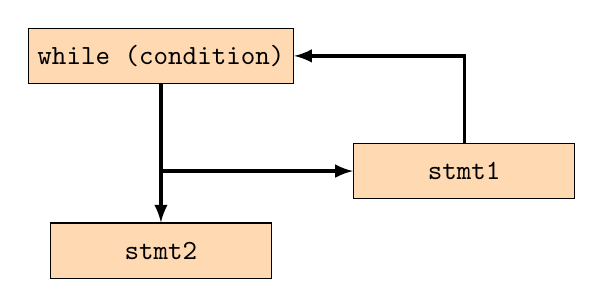
\begin{tikzpicture}[node distance = 9mm and 14mm,
  nodes= {draw, minimum width=8em, minimum height=2em,
    font=\ttfamily},
  startstop/.style = {fill=red!30, rounded corners},
  process/.style = {fill=orange!30},
  io/.style = {fill=blue!30,
    trapezium, trapezium stretches body,
    trapezium left angle=70, trapezium right angle=110},
  decision/.style = {fill=green!30, diamond, aspect=1.5},
  exp/.style={draw=none,font=\sffamily,minimum width=1em},
  arr/.style = {very thick,-latex}
  ]
  \node (while) [process] {while (condition)};
  \node (stmt1) [process,below right=3.0em of while] {stmt1};
  \node (stmt2) [process,below=5.0em of while] {stmt2};

  \draw[arr] (while) |- (stmt1);
  \draw[arr] (stmt1) |- (while);
  \draw[arr] (while) -- (stmt2);
\end{tikzpicture}
\end{document}
